\section{Utilizzo}

\subsection{Amministratore}

\subsubsection{Visualizzazione di una stanza}
\begin{figure}[H]
	\centering
	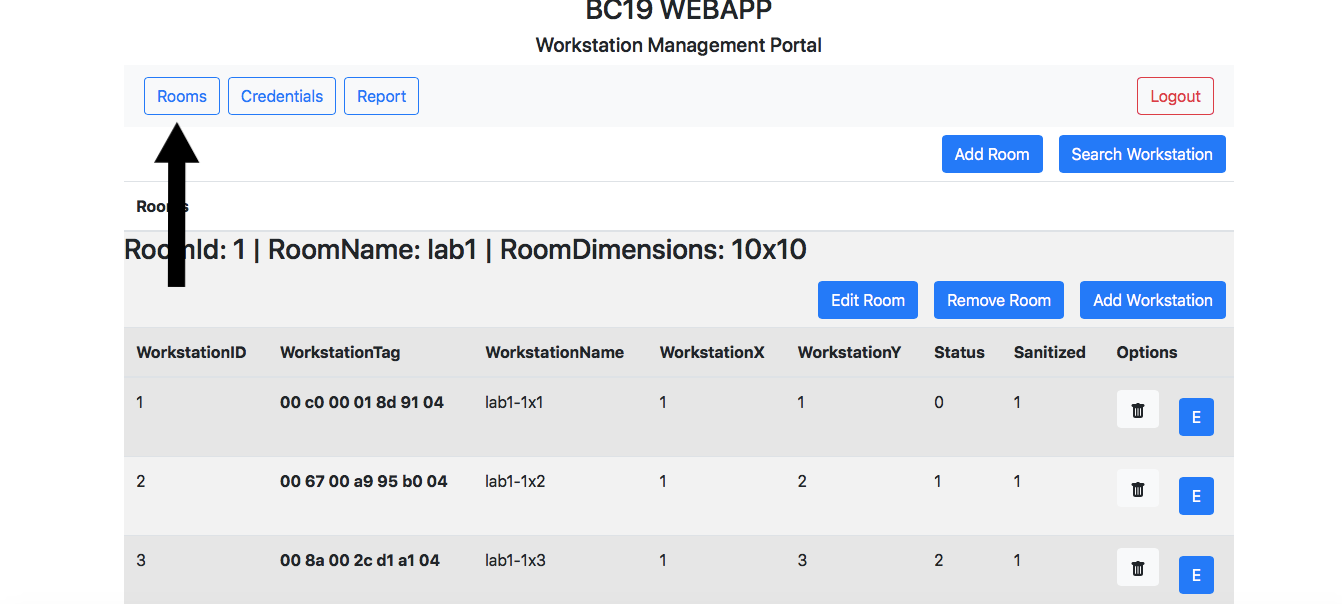
\includegraphics[width=15cm]{res/images/visStanza.png}
	\caption{Visualizzazione stanze}
\end{figure}
Per ogni stanza l'amministratore visualizza:
\begin{enumerate}
\item identificativo della stanza;
\item nome della stanza;
\item dimensioni della stanza.
\end{enumerate}
Per ogni postazione all'interno di una stanza l'amministratore visualizza:
\begin{enumerate}
\item identificativo della postazione;
\item identificativo del tag;
\item il nome della postazione;
\item l'ascissa della postazione nella stanza;
\item l'ordinata della postazione nella stanza;
\item lo stato della postazione;
\item lo stato dell' igienizzazione;
\item opzione per eliminare la postazione;
\item opzione per modificare la postazione.

\end{enumerate}

\subsubsection{Aggiunta di una stanza}
Per poter aggiungere una stanza, l'amministratore deve premere sul bottone 'Add Room'.
\begin{figure}[H]
	\centering
	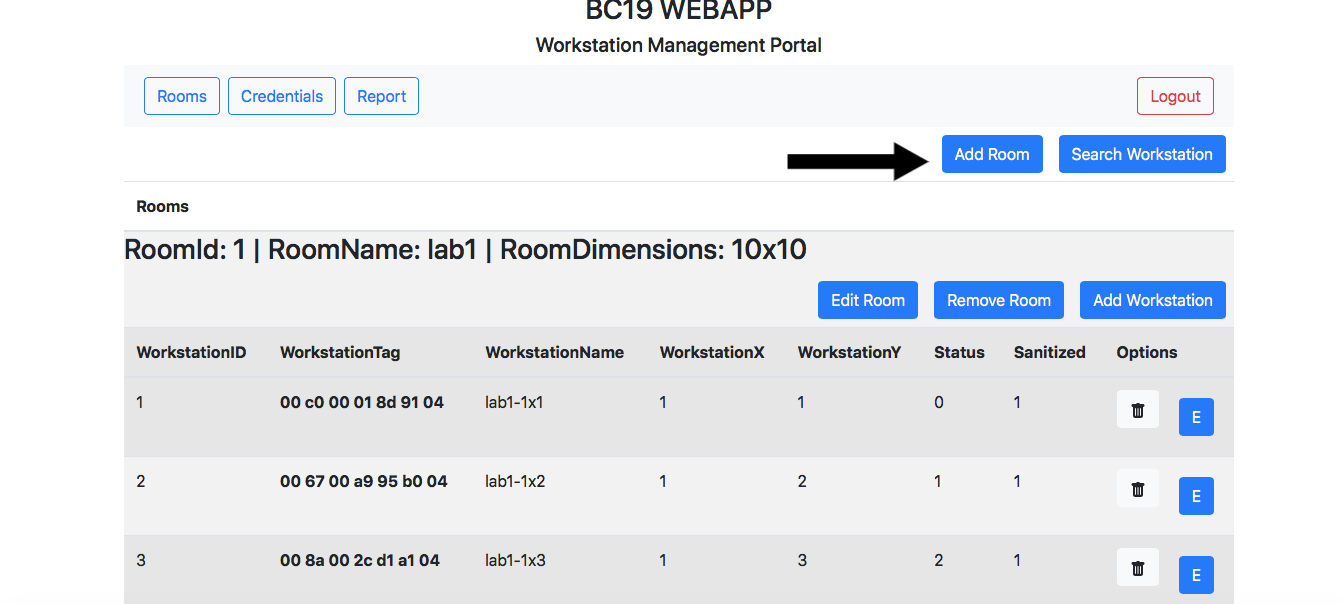
\includegraphics[width=15cm]{res/images/bottoneAddRoom.png}
	\caption{Visualizzazione bottoni}
\end{figure}
Una volta premuto sul bottone, comparirà un popup che l'amministratore dovrà compilare inserendo:
\begin{enumerate}
\item il nome della stanza;
\item la dimensione X;
\item la dimensione Y.
\end{enumerate}
\begin{figure}[H]
	\centering
	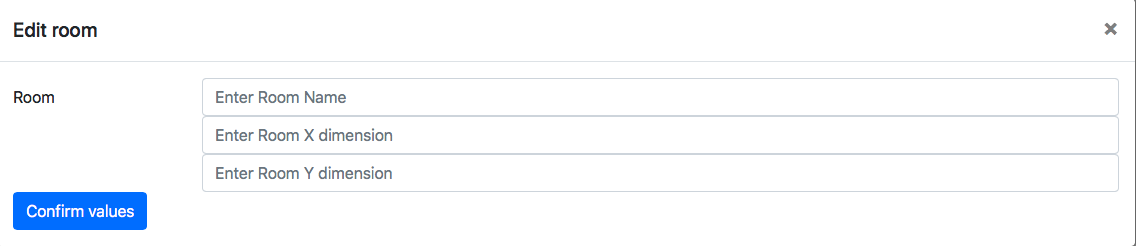
\includegraphics[width=15cm]{res/images/aggiungiStanza1.png}
	\caption{Visualizzazione popup aggiunta stanza}
\end{figure}

\subsubsection{Ricerca di una postazione}
Per poter ricercare una determinata postazione, l'amministratore deve premere sul bottone 'Search Workstation'.
\begin{figure}[H]
	\centering
	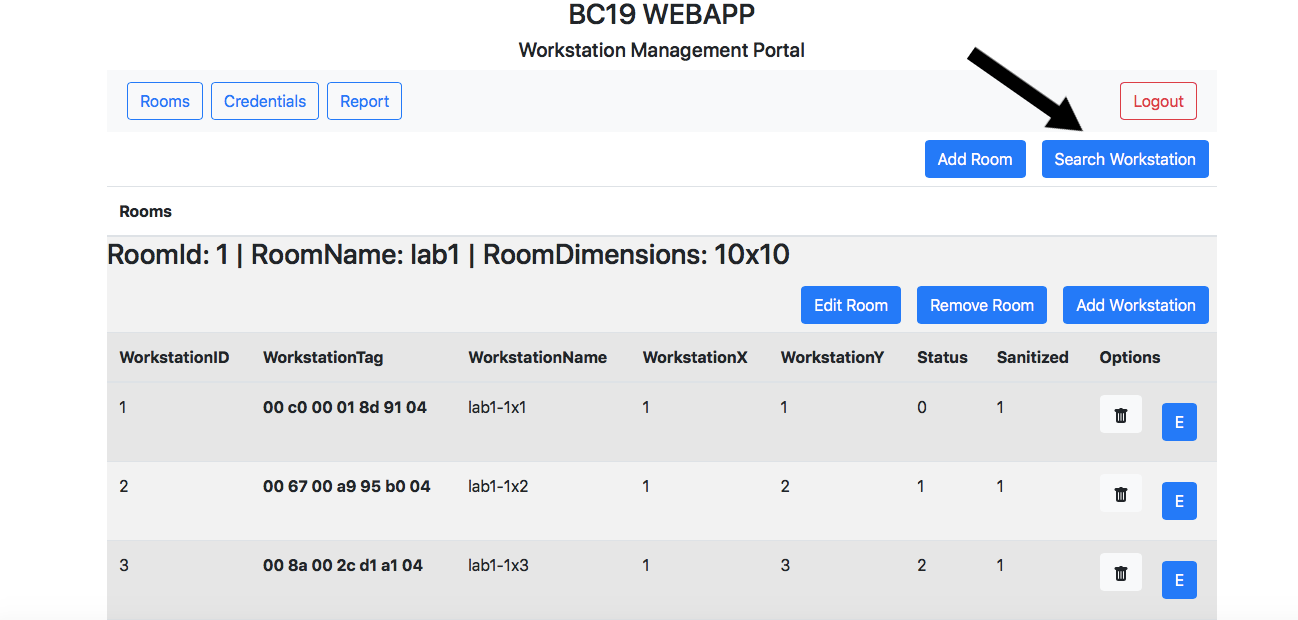
\includegraphics[width=15cm]{res/images/bottoneSearchWorkstation.png}
	\caption{Visualizzazione bottoni}
\end{figure}
Una volta premuto sul bottone, comparirà un popup che l'amministratore dovrà compilare inserendo:
\begin{enumerate}
\item l'identificativo della postazione;
Oppure
\item l'username di chi la occupa.
\end{enumerate}
\begin{figure}[H]
	\centering
	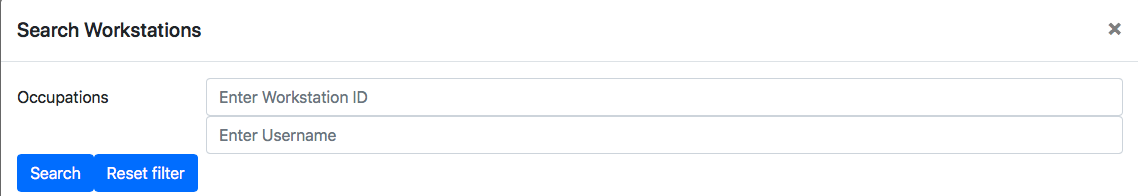
\includegraphics[width=15cm]{res/images/ricercaPostazione.png}
	\caption{Visualizzazione popup ricerca postazione}
\end{figure}

\subsubsection{Modifica di una stanza}
Per poter modificare le caratteristiche di una stanza, l'amministratore deve premere sul bottone 'Edit Room'.
\begin{figure}[H]
	\centering
	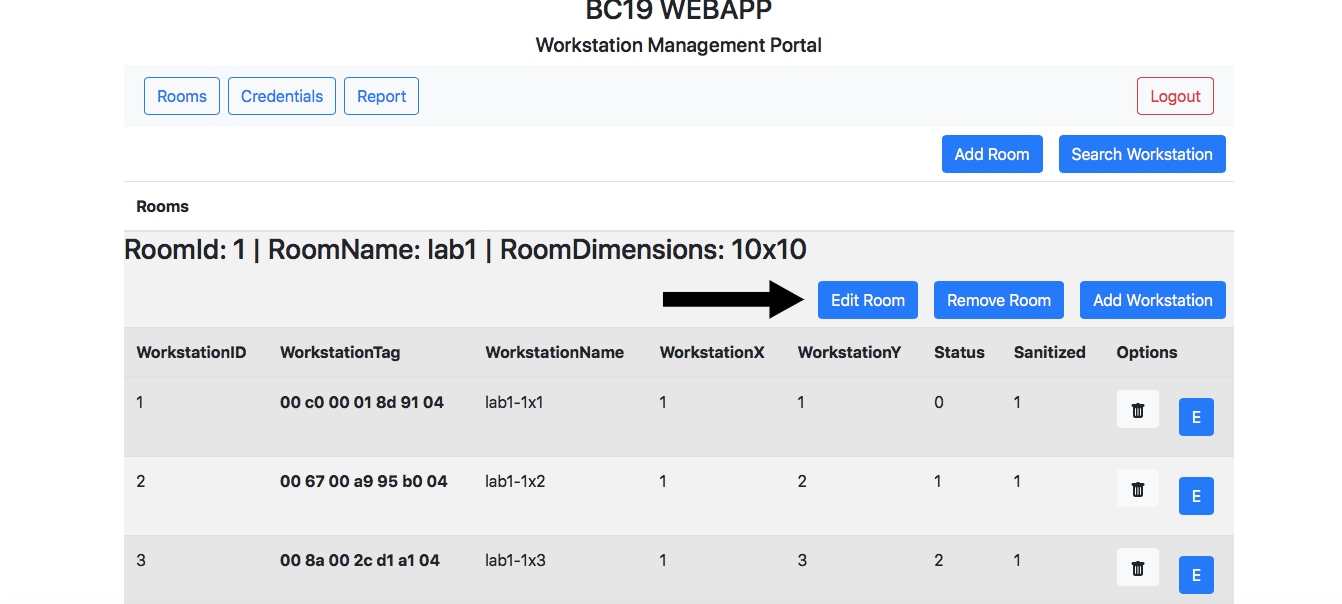
\includegraphics[width=15cm]{res/images/bottoneEditRoom.png}
	\caption{Visualizzazione bottoni}
\end{figure}
Una volta premuto sul bottone, comparirà un popup che l'amministratore dovrà compilare inserendo:
\begin{enumerate}
\item il nome della stanza;
\item la dimensione X;
\item la dimensione Y.
\end{enumerate}
\begin{figure}[H]
	\centering
	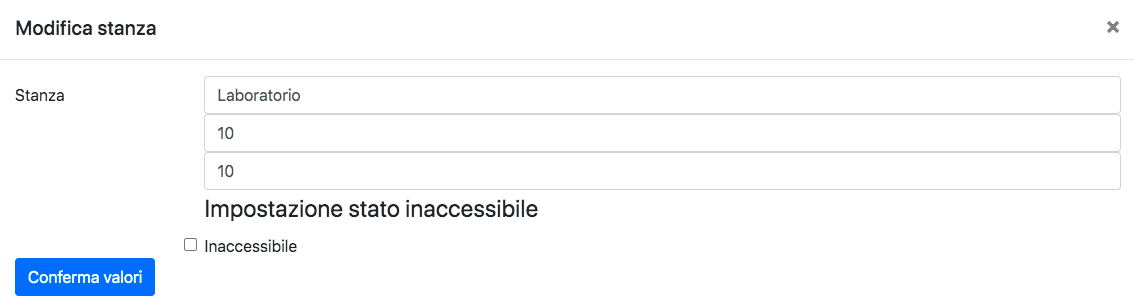
\includegraphics[width=15cm]{res/images/modificaStanza.png}
	\caption{Visualizzazione popup modifica stanza}
\end{figure}

\subsubsection{Rimozione di una stanza}
Per poter rimuovere una stanza, l'amministratore deve premere sul bottone 'Remove Room'.
\begin{figure}[H]
	\centering
	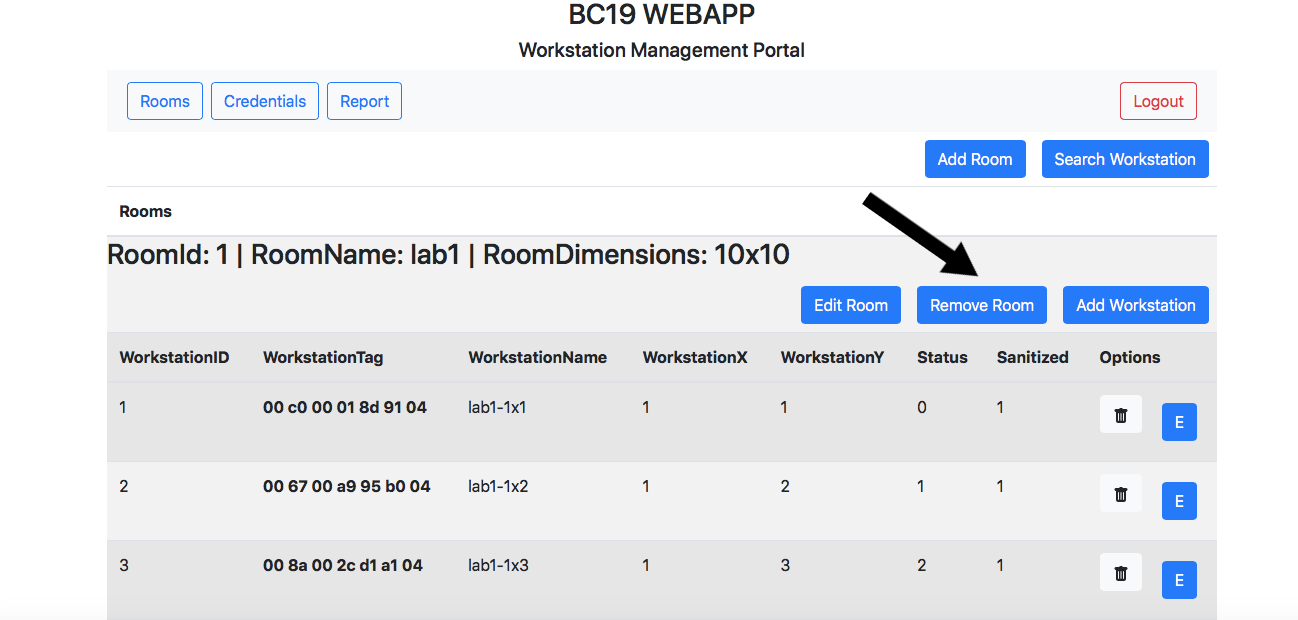
\includegraphics[width=15cm]{res/images/bottoneRemoveRoom.png}
	\caption{Visualizzazione bottoni}
\end{figure}
Una volta premuto sul bottone, comparirà un popup che chiederà all' amministratore una conferma per eliminare definitivamente la stanza.

\subsubsection{Aggiunta di una postazione all'interno di una stanza}
Per poter inserire una nuova postazione all'interno di una stanza, l'amministratore deve premere sul bottone 'Add Workstation'.
\begin{figure}[H]
	\centering
	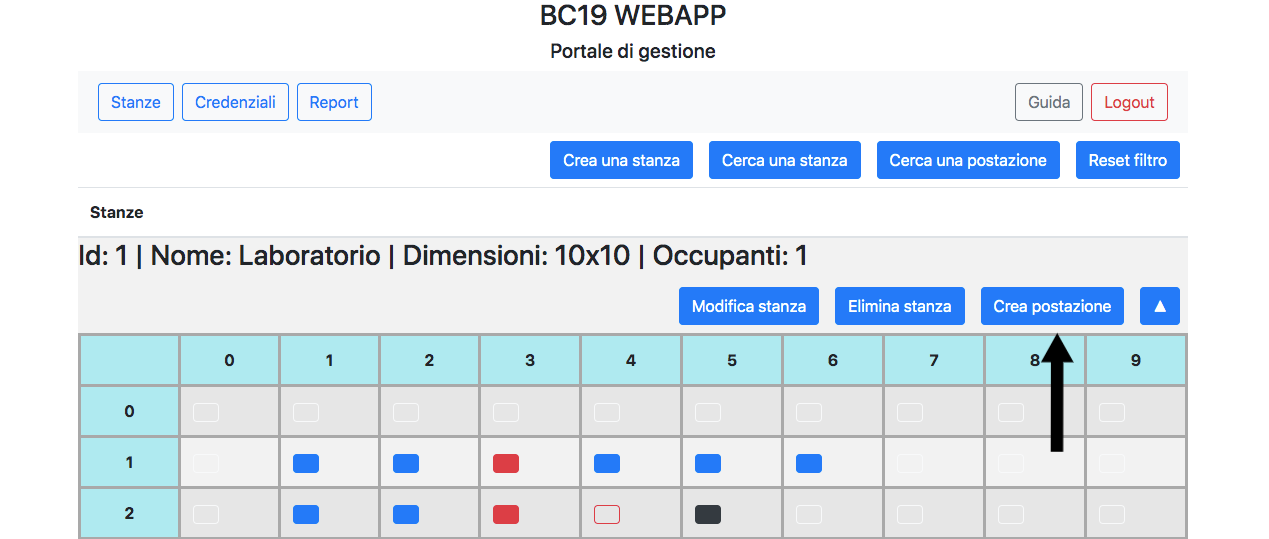
\includegraphics[width=15cm]{res/images/bottoneAddWorkstation.png}
	\caption{Visualizzazione bottoni}
\end{figure}
Una volta premuto sul bottone, comparirà un popup che l'amministratore dovrà compilare inserendo:
\begin{enumerate}
\item il tag della postazione;
\item il nome della postazione;
\item la dimensione X della postazione nella stanza;
\item la dimensione Y della postazione nella stanza.
\end{enumerate}
\begin{figure}[H]
	\centering
	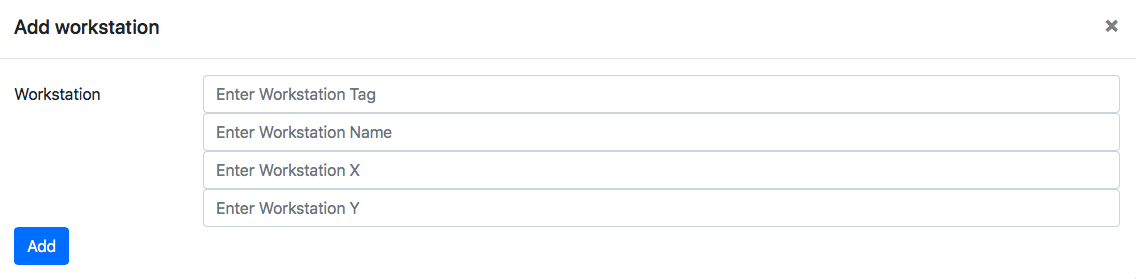
\includegraphics[width=15cm]{res/images/addWorkstation.png}
	\caption{Visualizzazione popup inserimento postazione dentro a una stanza}
\end{figure}

\subsubsection{Eliminazione di una postazione all'interno di una stanza}
Per poter eliminare una postazione all'interno di una stanza, l'amministratore deve premere sul bottone dove è raffigurato un cestino.
\begin{figure}[H]
	\centering
	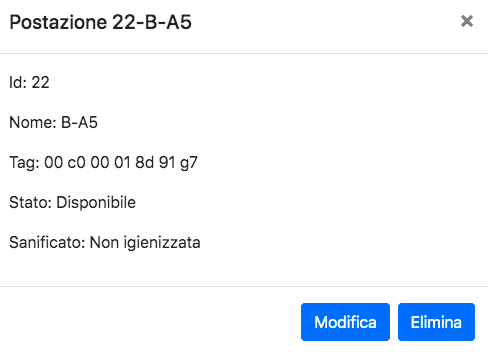
\includegraphics[width=15cm]{res/images/bottoneCestinoWorkstation.png}
	\caption{Visualizzazione bottoni}
\end{figure}
Una volta premuto sul bottone, comparirà un popup che chiederà all' amministratore una conferma per eliminare definitivamente la postazione dentro alla stanza.

\subsubsection{Modifica di una postazione all'interno di una stanza}
Per poter modificare le caratteristiche di una postazione all'interno di una stanza, l'amministratore deve premere sul bottone 'E' di colore blu.
\begin{figure}[H]
	\centering
	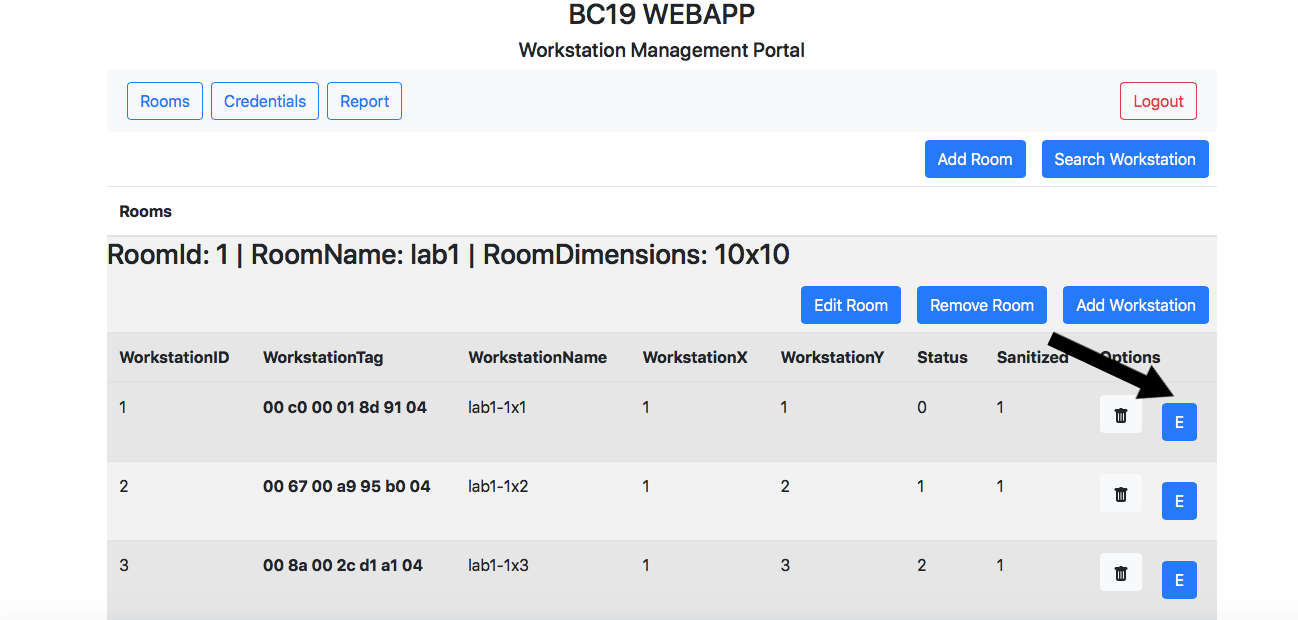
\includegraphics[width=15cm]{res/images/bottoneEditWorkstation.png}
	\caption{Visualizzazione bottoni}
\end{figure}
Una volta premuto sul bottone, comparirà un popup che l'amministratore dovrà compilare inserendo:
\begin{enumerate}
\item il tag della postazione;
\item il nome della postazione;
\item la dimensione X della postazione nella stanza;
\item la dimensione Y della postazione nella stanza.
\end{enumerate}
\begin{figure}[H]
	\centering
	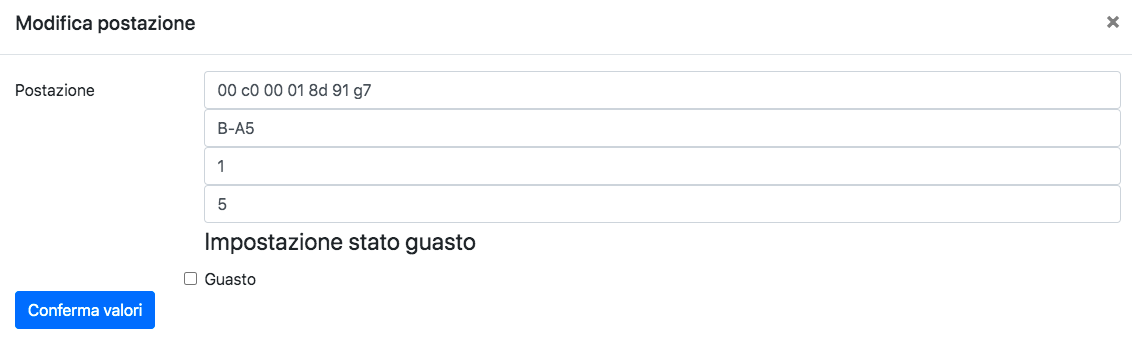
\includegraphics[width=15cm]{res/images/editWorkstation.png}
	\caption{Visualizzazione popup modifica postazione all'interno di una stanza}
\end{figure}

\subsection{Dipendente}
L'applicazione mobile viene utilizzata dagli utenti che vogliono accedere ad una postazione di una stanza dell'organizzazione. Essi hanno la possibilità di effettuare una prenotazione e di conoscere lo stato di una postazione, tramite la scansione del tag NFC associato. Inoltre per ogni occupazione viene registrato l'orario di inizio e di fine, e monitorata la presenza in tempo reale da parte dell'amministratore. Inoltre, ogni utente ha la possibilità di effettuare un'igienizzazione di una postazione precedentemente utilizzata. 
\\All'utente dell'applicazione vengono offerte tutte le funzionalità indicate in questa sezione.
\subsubsection{Login}
\begin{figure}[H]
	\centering
	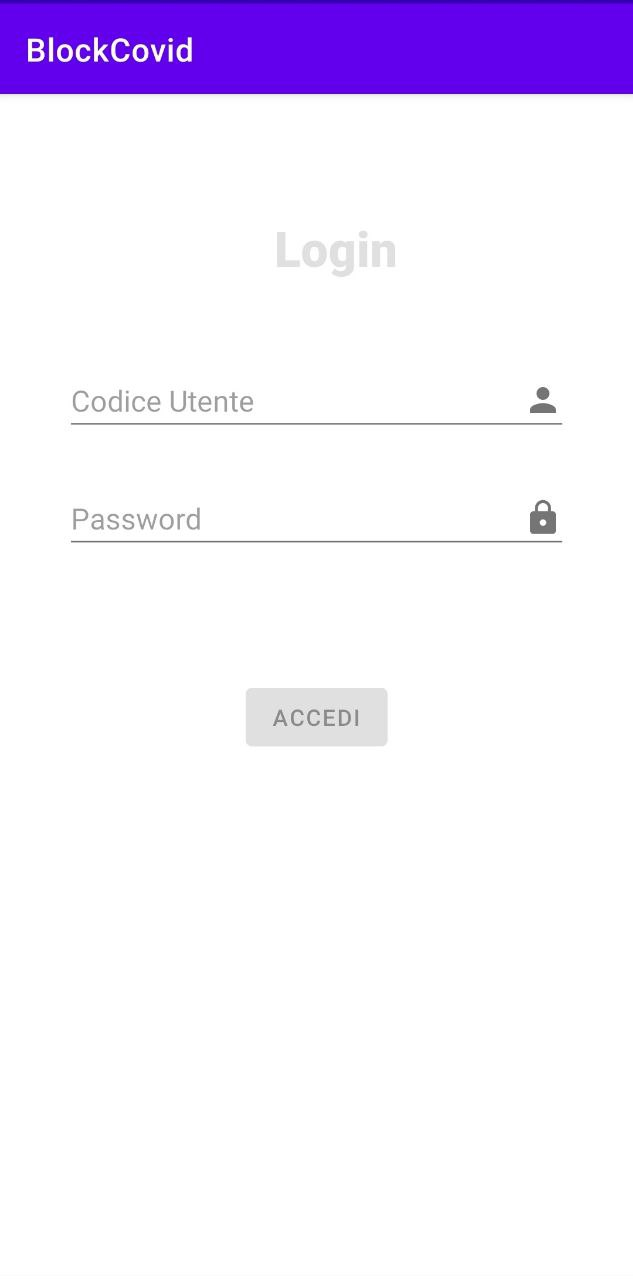
\includegraphics[width=5cm]{res/images/login.png}
	\caption{Login utente}
\end{figure}
L'utente può autenticarsi nella pagina iniziale del login inserendo il proprio username e la propria password nelle EditText corrispondenti.
Nel caso in cui inserisca le credenziali corrette otterrà l'accesso all'applicazione e quindi alla pagina principale, altrimenti verrà visualizzato un messaggio di errore in cui verrà comunicato di riprovare il login.

\subsubsection{Logout}
\begin{figure}[H]
	\centering
	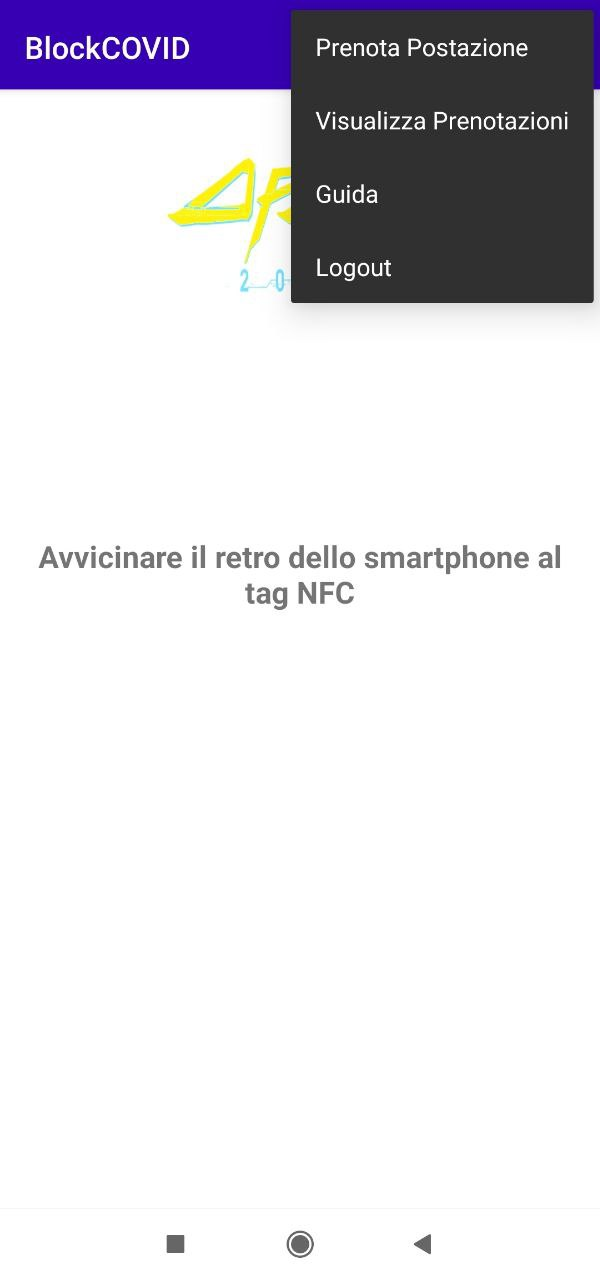
\includegraphics[width=5cm]{res/images/menuATendina.png}
	\caption{Logout utente}
\end{figure}
L'utente può eseguire il logout aprendo il menù a tendina in alto a destra e poi cliccando su logout. Avvenuta questa operazione l'utente si troverà nella pagina del login.

\subsubsection{Scansione tag NFC}
\begin{figure}[H]
	\centering
	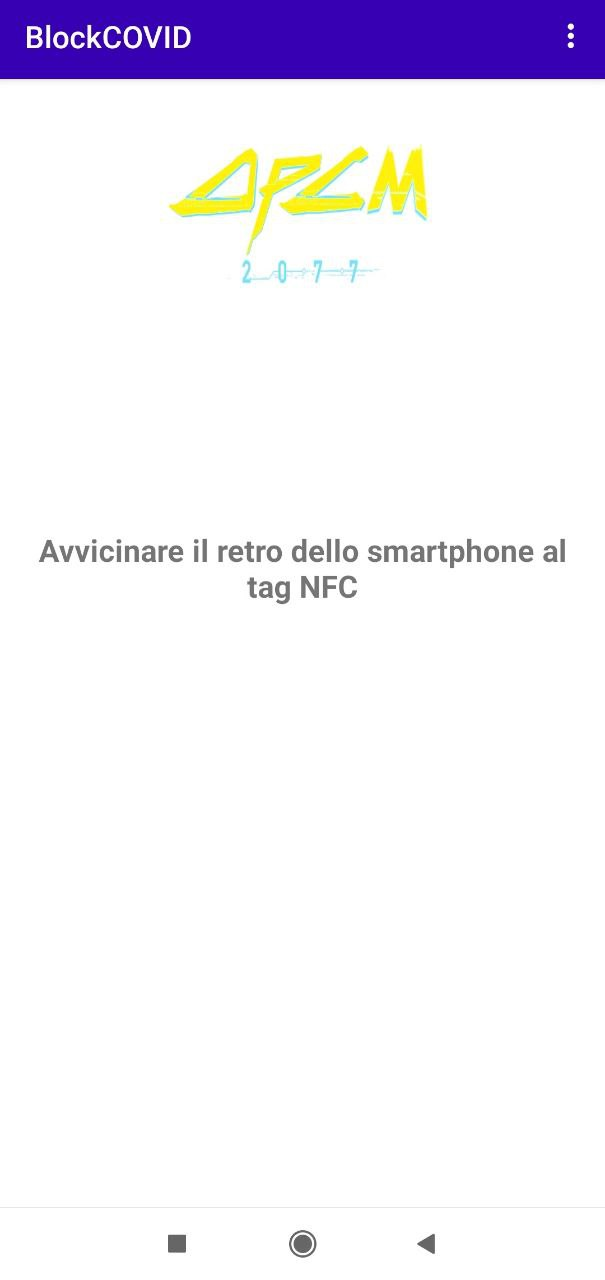
\includegraphics[width=5cm]{res/images/avvicinaSmartphone.png}
	\caption{Scansione tagNFC}
\end{figure}
L'utente si trova nella pagina principale dell'applicazione e gli viene chiesto di effettuare una scansione del tag NFC tramite lo smartphone. 
\subsubsection{Visualizzazione stato postazione}
\begin{figure}[H]
	\centering
	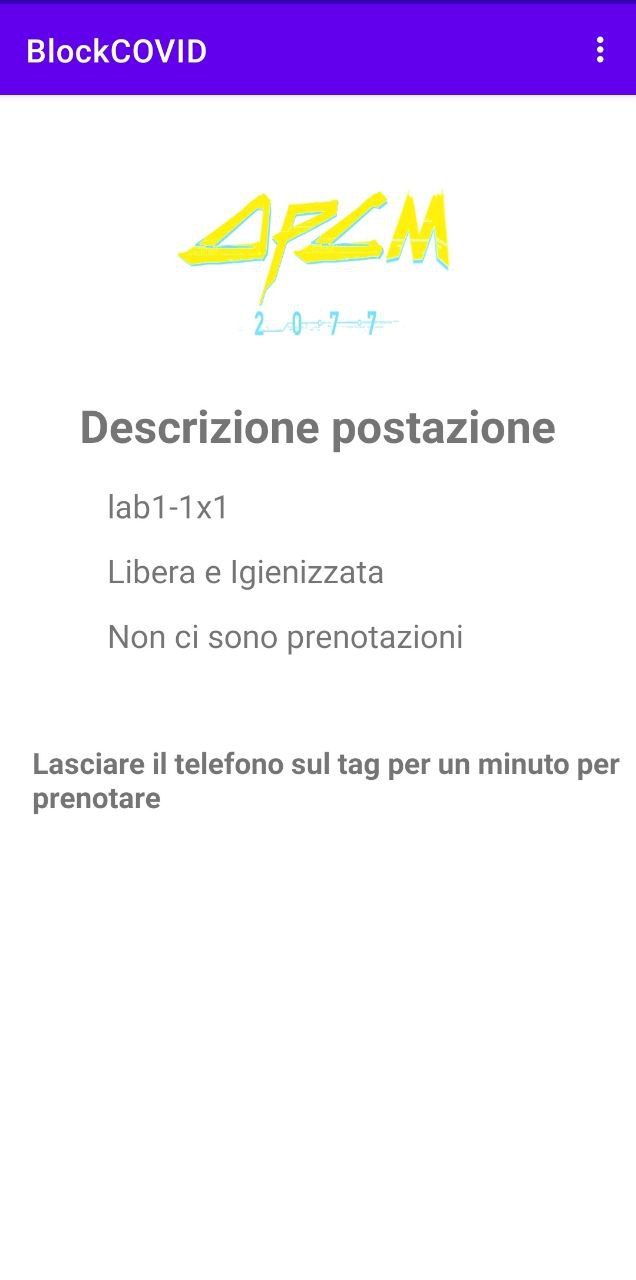
\includegraphics[width=5cm]{res/images/DescrizionePostazione1.png}
	\caption{Stato postazione}
\end{figure}
L'utente ha effettuato la scansione di una postazione e riceve le seguenti informazioni nella pagina principale dell'applicazione:
\begin{itemize}
	\item stanza della prenotazione e posizione indicata tramite X e Y;
	\item stato della postazione;
	\item eventuale nome del dipendente che ha prenotato la postazione.
\end{itemize}
In base allo stato in cui si trova la postazione, l'utente visualizzerà un messaggio differente:
\begin{itemize}
	\item se libera e igienizzata, si invita l'utente a lasciare il telefono sul tag NFC per effettuare una prenotazione automatica della postazione;
	\item se libera e non igienizzata, si invita l'utente ad effettuare la pulizia autonoma della postazione tramite il kit aziendale e quindi di cliccare il bottone "igienizza";
	\item se prenotata e igienizzata, si invita l'utente ad abbandonare la postazione dato che al momento non è disponibile;
	\item se prenotata e non igienizzata, si invita l'utente ad effettuare la pulizia autonoma della postazione tramite il kit aziendale e quindi di cliccare il bottone "igienizza";
	\item se guasta e igienizzata, si invita l'utente ad abbandonare la postazione dato che al momento non è disponibile;
	\item se guasta e non igienizzata, si invita l'utente ad effettuare la pulizia autonoma della postazione tramite il kit aziendale e quindi di cliccare il bottone "igienizza";
\end{itemize}
 
\subsubsection{Occupazione postazione}
\begin{figure}[H]
	\centering
	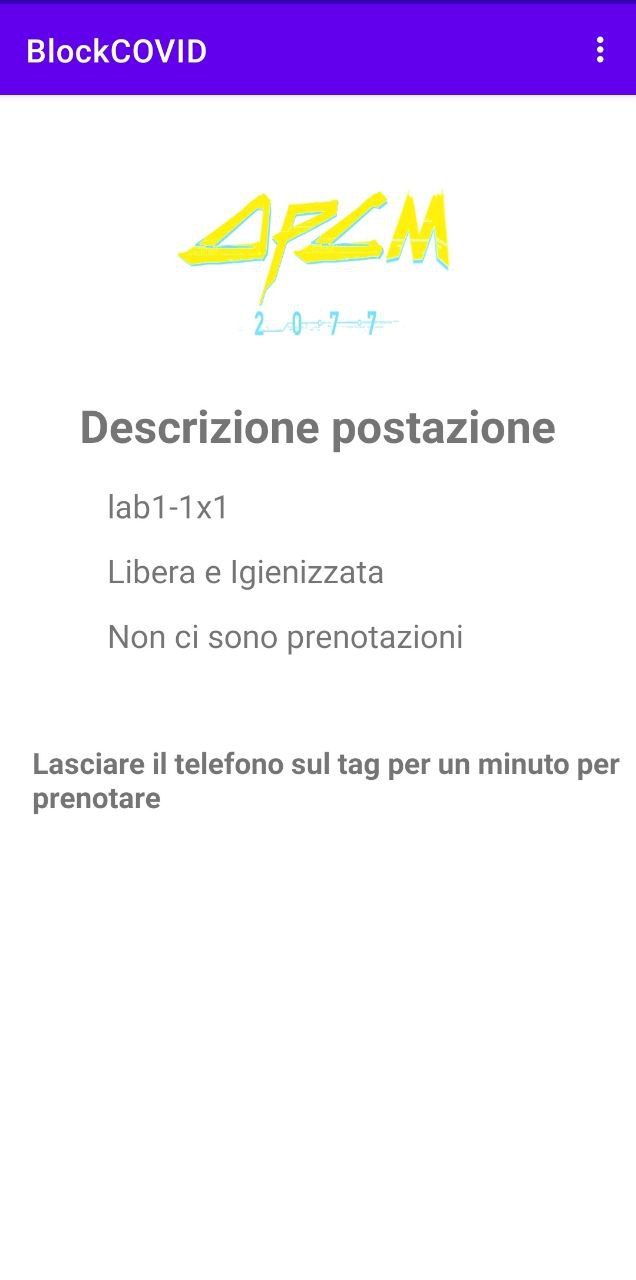
\includegraphics[width=5cm]{res/images/DescrizionePostazione1.png}
	\caption{Inizio occupazione postazione}
\end{figure}
L'utente dopo aver scansionato con il proprio smartphone il tag NFC per un tempo maggiore o uguale ad un minuto, prenota in modo automatico la postazione per
l’intera giornata lavorativa. Lo stato della postazione deve essere libera e igienizzata e non prenotata da un altro utente durante il resto della giornata.
\subsubsection{Igienizzazione postazione}
\begin{figure}[H]
	\centering
	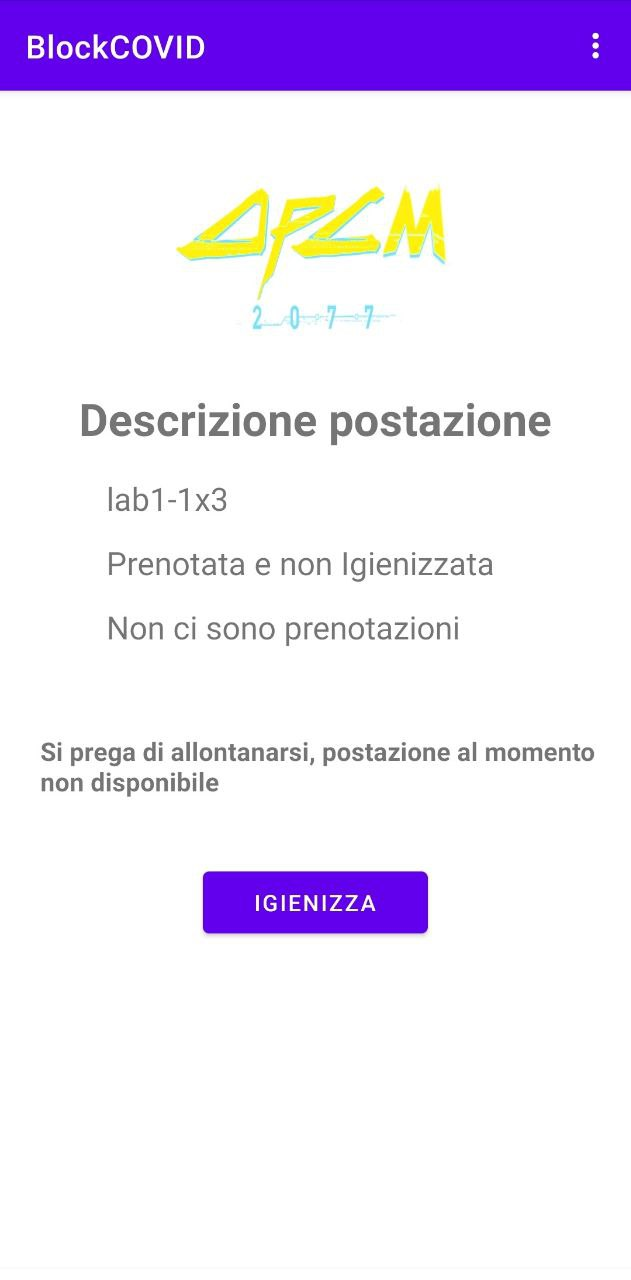
\includegraphics[width=5cm]{res/images/DescrizionePostazione3.png}
	\caption{Igienizzazione postazione}
\end{figure}
L'utente igienizza una postazione il cui stato è diverso da "igienizzato" e lo segnala premendo l'apposito bottone "igienizza" nella pagina principale dell'applicazione. In modo automatico lo stato della postazione viene registrato come libera e igienizzata, prenotata e igienizzata o guasta e igienizzata.
\subsubsection{Visualizzazione lista prenotazioni}
\begin{figure}[H]
	\centering
	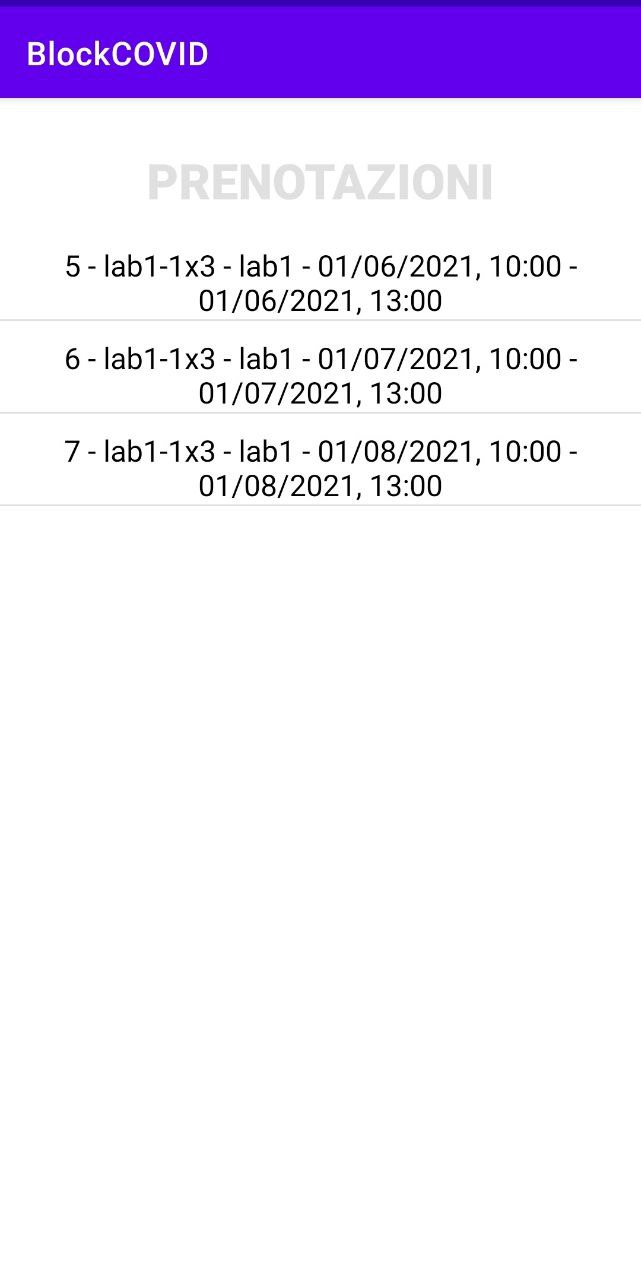
\includegraphics[width=5cm]{res/images/VisualizzaPrenotazioni.png}
	\caption{Visualizzazione lista prenotazioni}
\end{figure}
L’utente può accedere alla sezione per la visualizzazione della lista delle prenotazioni da lui effettuate, cliccando il menù a tendina in alto a destra.
Ogni postazione mostra le seguenti informazioni:
\begin{itemize}
	\item stanza della prenotazione;
	\item posizione indicata tramite X e Y;
	\item data/ora di inizio della prenotazione;
	\item data/ora di fine della prenotazione.
\end{itemize}
\subsubsection{Disdetta prenotazione}
\begin{figure}[H]
	\centering
	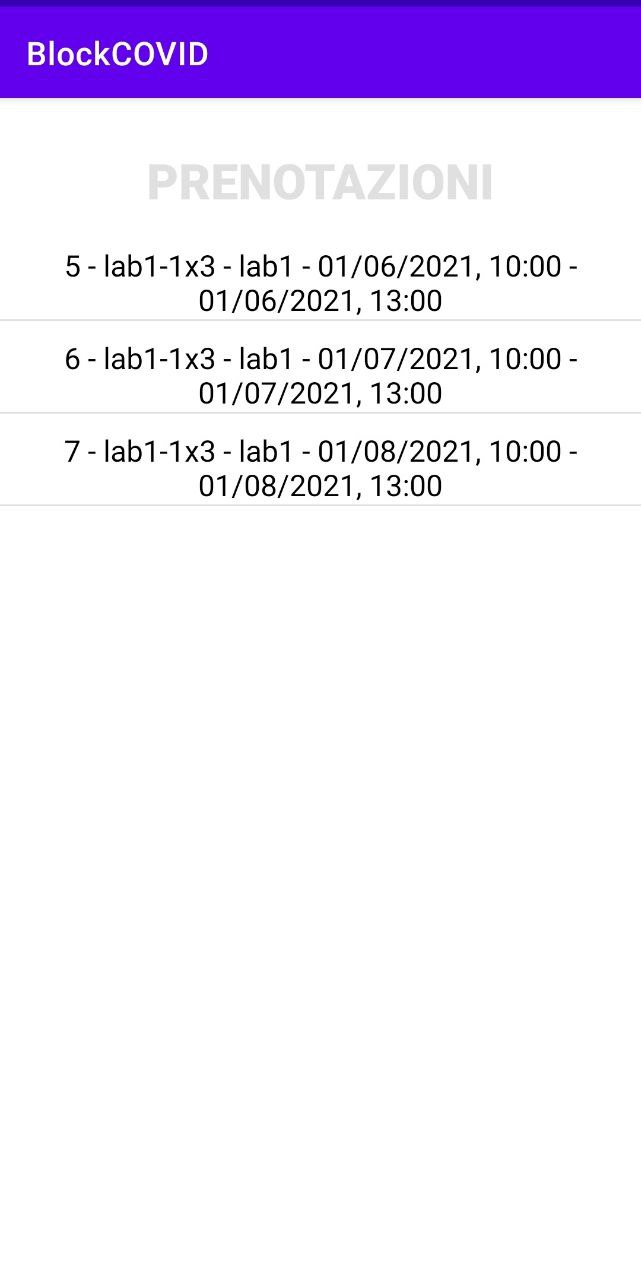
\includegraphics[width=5cm]{res/images/VisualizzaPrenotazioni.png}
	\caption{Disdetta prenotazione}
\end{figure}
L’utente si trova nella sezione di visualizzazione della lista delle prenotazioni, arrivatoci cliccando il menù a tendina in alto a destra, e disdice una prenotazione da lui effettuata in precedenza.
\subsubsection{Guida utente}
\begin{figure}[H]
	\centering
	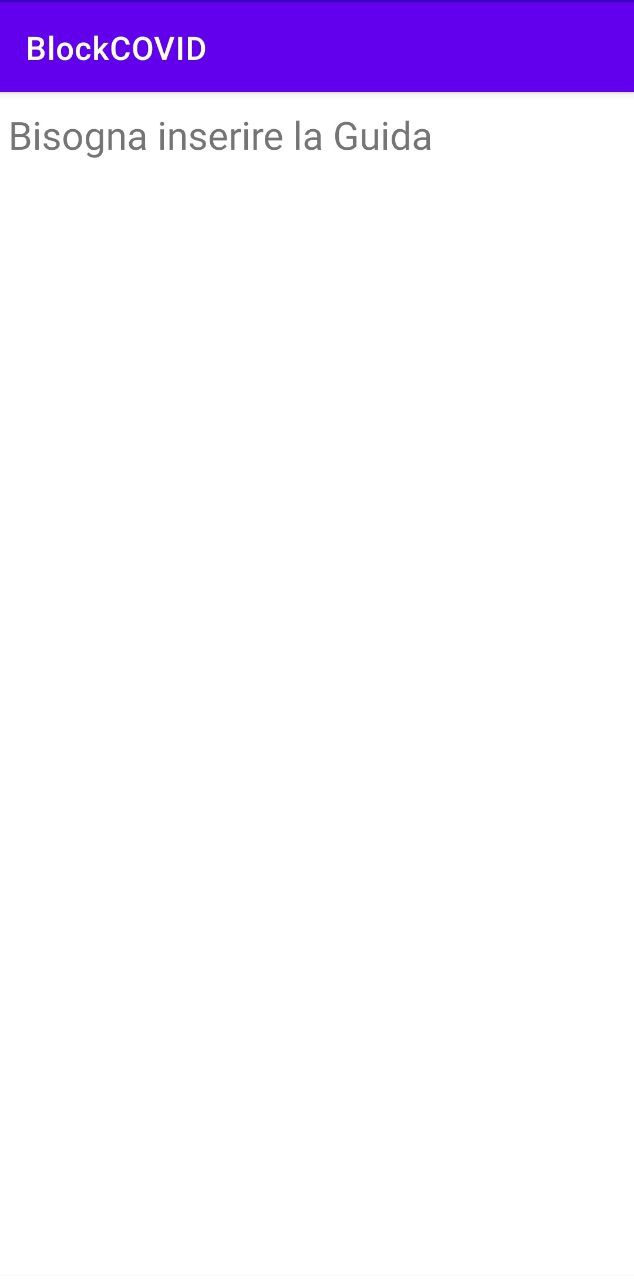
\includegraphics[width=5cm]{res/images/Guida.png}
	\caption{Guida dipendente}
\end{figure}
L’utente accede alla pagina Guida utente, cliccando la sezione apposita del menù a tendina in alto a destra, e riceve una guida riguardo le funzionalità principali dell'applicazione.
\subsubsection{Prenotazione postazione}
\begin{figure}[H]
	\centering
	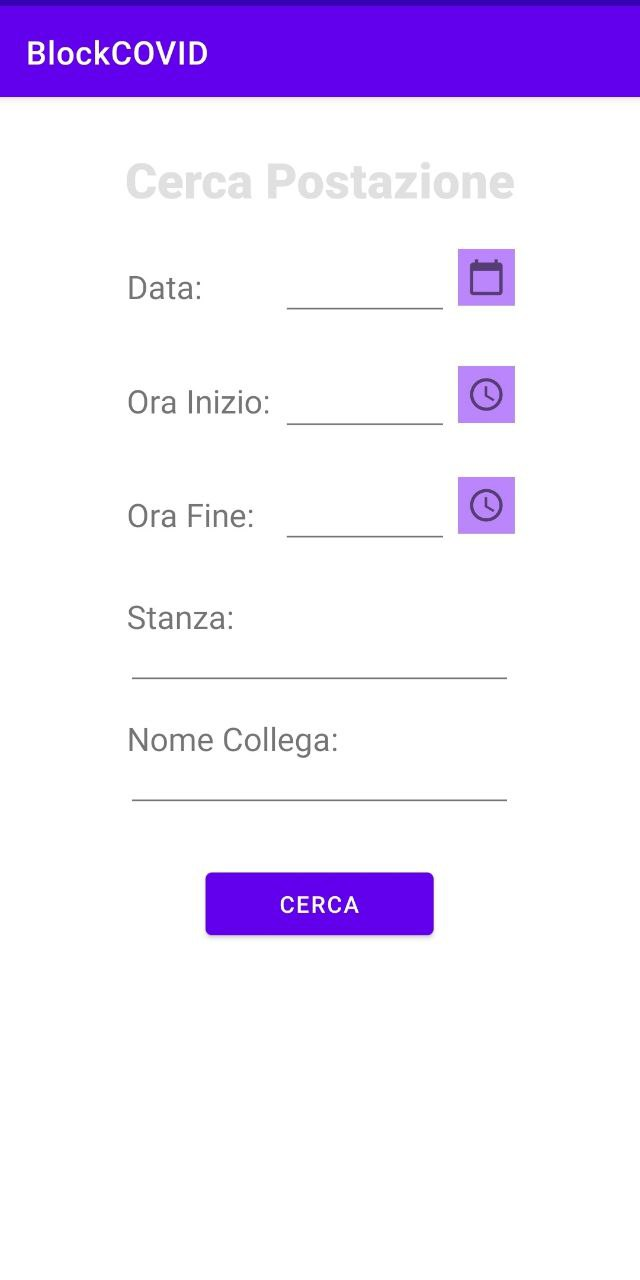
\includegraphics[width=5cm]{res/images/PrenotaPostazione.png}
	\caption{Prenotazione postazione}
\end{figure}
Il dipendente può prenotare una postazione premendo sull'elemento della lista "Prenota postazione" del menù principale in alto a destra.
Dopo aver premuto dovrà inserire la data, l'ora di inizio, l'ora di fine e la stanza obbligatoriamente e in modo facoltativo anche il nome del collega. Per facilitare l'utente nell'inserimento dei dati, a destra di ciascun EditText è presente una GUI per la selezione di una data(vista a calendario) e di un orario(vista a orologio). Una volta premuto sul bottone "Cerca", se è stato inserito il nome del collega, visualizzerà tutte le sue prenotazioni effettuate nella stanza, nel range orario e nella data inseriti e scorrendo sotto visualizzerà tutte le postazioni di quella stanza con il loro stato e potrà decidere quale prenotare se disponibile. 




\subsection{Addetto alle pulizie}